\chapter{Correlations Analysis}
\label{chpr:ch3}
\bigskip

A correlation analysis is needed to assess the properties of cryptoassets in an investment portfolio. From here on we refer to logarithmic returns simply as returns.

\section{Empirical Correlations}
First of all, we calculate the empirical correlation between all the instruments in the portfolio based on the empirical time series of our dataset.
For this part, we will consider our data as successive samples of a N-dimensional vector in RN, where N is the number of assets:
\begin{equation}
    \text{x}_j = \left( \begin{array}{c}
         x_{1,j} \\
         x_{2,j} \\
         .\\
         .\\
         .\\
         x_{N,j}
    \end{array} \right) , j = 1...N_{sample}
\end{equation}

Each element $i$ of the vector $\text{x}_j$ represents the $j^{th}$ realization of the returns for asset $i$.
Following basic statistics, we can now compute the sample mean of our vectors of returns as:
\begin{equation}
    \Bar{\text{x}} = \frac{1}{N_{sample}} \sum_{{j = 1}}^{N_{sample}} \text{x}_j = \left( \begin{array}{c}
         \Bar{x}_1 \\
         \Bar{x}_2 \\
         .\\
         .\\
         .\\
         \Bar{x}_N
    \end{array} \right)
\end{equation}

where $\Bar{\text{x}}_i = \frac{1}{N_{sample}} \sum_{{j = 1}}^{N_{sample}} x_{i,j}$ is the sample mean of component $i$.

\noindent
We then compute the sample covariance matrix through the following formula:
\begin{equation}
    \Bar{\Sigma} = \frac{1}{N_{sample}-1} \sum_{{j = 1}}^{N_{sample}} \left( \text{x}_j - \Bar{\text{x}} \right) \left( \text{x}_j - \Bar{\text{x}} \right)^T
\end{equation}

where $\Bar{x}$ represent the sample mean of the returns just introduced. All the information needed to obtain the correlation matrix $C$ are already included in $\Bar{\Sigma}$, we only need to perform some further calculations:

\begin{equation}
    C_{i,j} = \frac{\Bar{\Sigma}_{i,j}}{\sqrt{\Bar{\Sigma}_{i,i}\Bar{\Sigma}_{j,j}}}
\end{equation}

We have thus obtained an empirical estimate of the correlation between our assets returns. The formula of $C_{i,j}$ is often referred to as Pearson correlation coefficient, from the name of the English mathematician Karl Pearson who first formulated it.

See below the table with expected returns and volatility of returns:

\begin{table}[H]
   \begin{tabular}{c | c c}
         & Annualized Mean Return & Annualized Mean Volatility\\ \hline
        btc & 131.09\% & 72.73\%\\
        eth & 395.64\% & 120.92\%\\
        ltc & 161.96\% & 109.69\%\\
        xrp & 231.37\% & 129.85\%\\
        bric & 9.10\% & 15.61\%\\
        sp500 & 10.27\% & 12.58\%\\
        eurostoxx & 1.66\% & 15.51\%\\
        nasdaq & 13.62\% & 15.75\%\\
        bond\_europe & 1.52\% & 2.90\%\\
        bond\_us & 2.85\% & 2.83\%\\
        bond\_eur & 2.08\% & 2.47\%\\
        eur & 0.91\% & 7.32\%\\
        gbp & -4.18\% & 10.36\%\\
        chf & -0.01\% & 6.88\%\\
        jpy & 2.81\% & 9.03\%\\
        gold & 5.28\% & 11.66\%\\
        wti & 14.39\% & 33.78\%\\
        grain & -8.70\% & 17.44\%\\
        metal & 6.03\% & 15.47\%\\
        \hline
    \end{tabular}
    \caption{Annualized Mean Returns and Variances}
\end{table}
\bigskip
And then the correlation matrix:

\begin{figure}[H]
    \centering
    \makebox[\textwidth][c]{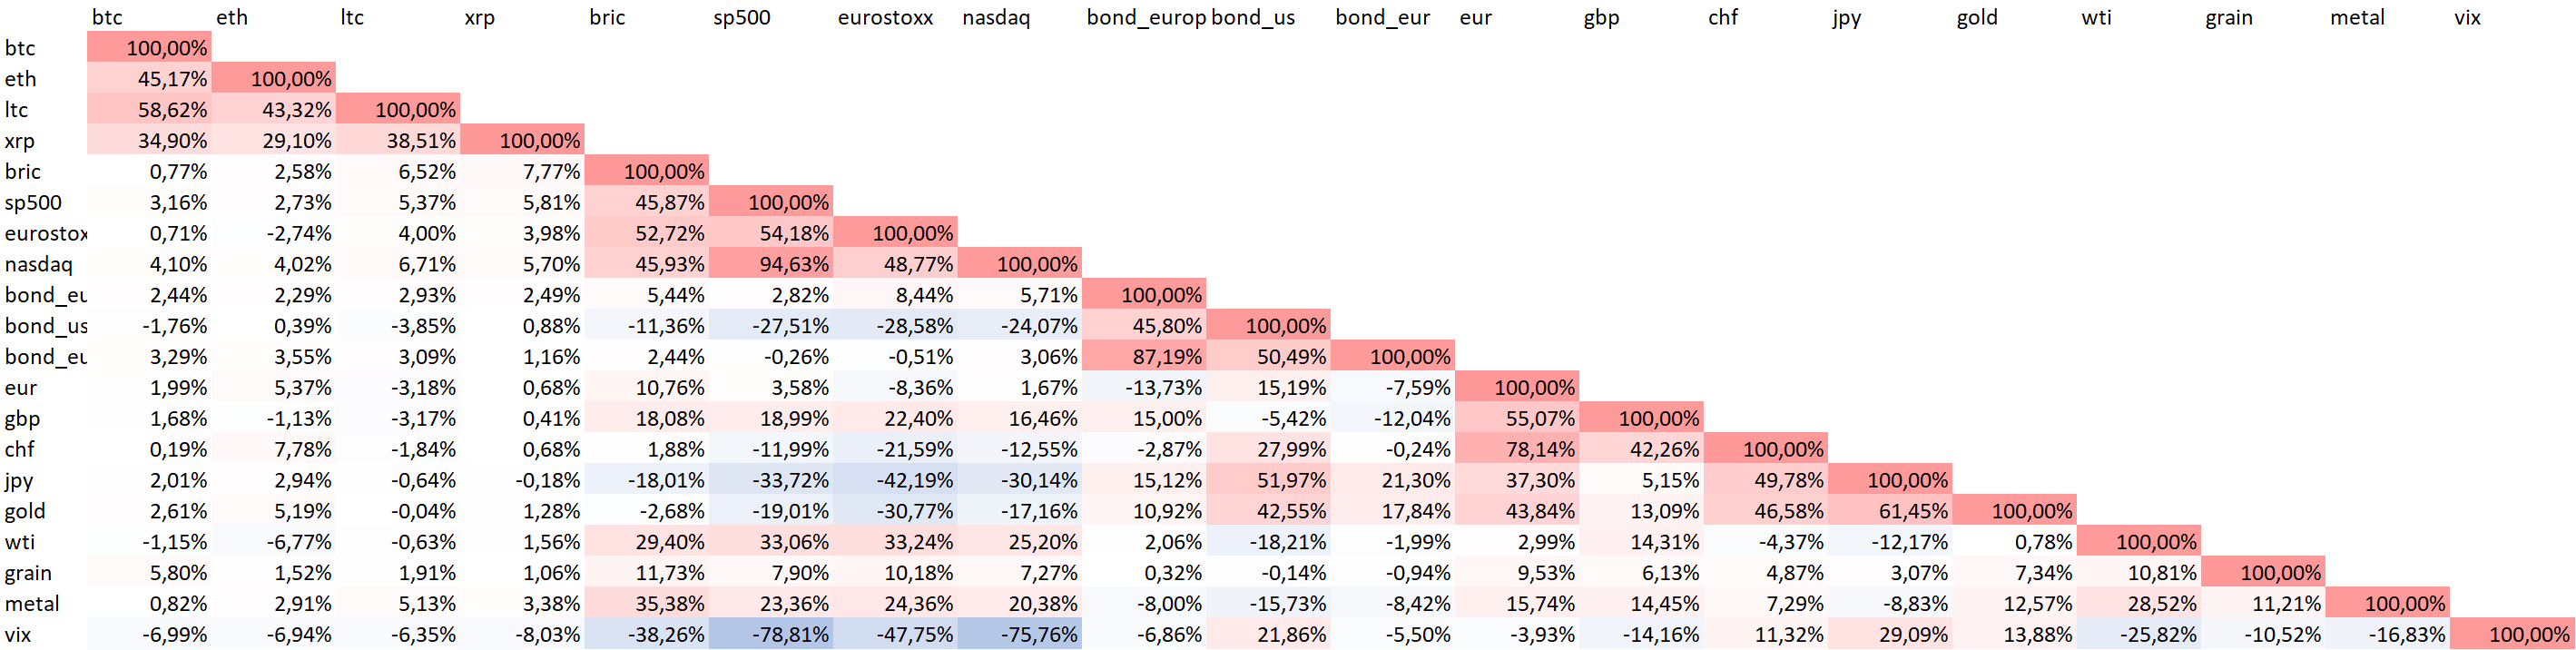
\includegraphics[width=15.5cm, height=5cm]{Images/corr_tot.png}}
    \caption{Historical correlations matrix}
\end{figure}
\bigskip

There are mainly two things that we may notice. First of all, we can see very low correlation between the cryptoassets and all the other instruments: none of these correlations is double digit and almost all of them are below 5\% in absolute value. On the contrary, inside the “world” of the cryptoassets, correlations are much higher.

\noindent
To better analyse the first point, we proceed by performing a statistical test on the correlation values between each cryptoasset and other instruments.

\section{Correlation Significance}

We would investigate whether it is correct to assume that the cryptoasset world is uncorrelated with all the other instruments. If it will be the case this would mean that investing in cryptoassets could improve a portfolio in terms of diversification.

\noindent
We will perform an hypothesis test. In particular we are interested in testing if the sample correlation coefficients are significantly different from zero or not. Both of the following tests are presented in the most general form for a sample of two variables, with their distribution correlation ρ and their sample correlation $\hat{\rho}$.

Following standard testing procedure, we specify the null hypothesis and the alternative hypothesis:
\begin{equation}
    \text{H}_0 : \rho = 0 \quad  vs. \quad \text{H}_1 : \rho \neq 0.
\end{equation}

\noindent
These will be common to both presented tests which are the \textit{Pearson's t-test} and the \textit{Permutation test}.

\subsection{Pearson's t-test}
Our first test is based on Student’s t-distribution and the following t-statistic:
\begin{equation}
    t= \hat{\rho} \sqrt{\frac{n-2}{1-\hat{\rho}^2}},
\end{equation}

which under the null hypothesis is distributed as a Student’s t with n-2 degrees of freedom, where n stands for the cardinality of the sample. We can thus proceed by computing the relative p-value and compare it to a given level of confidence α (usually $\alpha$ = 95\%). The result of the test will be deduced as follows:
\begin{itemize}
    \item $p-value < 1-\alpha$: we have statistical evidence to state that the correlation is significantly different from zero;
    \item $p-value \geq 1-\alpha$:there is no statistical evidence to state that the correlation is significantly different from zero.
\end{itemize}

\subsection{Permutation test}
The permutation test is based on building an empirical distribution of values for the correlation by sampling different pairs of $X$ and $Y$ variable and then computing Pearson’s correlation. Let $\left( x_i, y_i \right)$ be the original pairs for $i = 1,…,N_{sample}$. Create a new dataset $\left(x_i, y_i^*\right)$ by replacing $y_i$ with one of the possible $N_{sample}$ permutations and then compute the new sample correlation for the new dataset. If this is done a large enough number of times, we obtain an empirical distribution of possible values for the correlation of $x$ and $y$.
From this distribution we can then obtain the $p-value$ of the test and thus get the final result in the same way as in the previous case.

\subsection{Significance results}
Here we report the first results of our analysis: in tables \ref{tante1}, \ref{tante2}, \ref{tante3} and \ref{tante4} there are the values and relative $p-values$, given from Pearson $t-test$ and permutation test, of the correlations between these 4 cryptoassets and the indexes.

\noindent
One can immediately notices that very few correlations are above $0.05$ or below $-0.05$ and no one is above $0.10$ or below $-0.10$. Moreover the $p-Values$ are in general high enough to reject the alternative hypothesis and when this is not the case the correlation is still considerably low.

\begin{table}[H]
   \resizebox{\textwidth}{!}{\begin{tabular}{c c | c c c c c c c}
        && bric & sp500 & eurostoxx & nasdaq & bond\_europe & bond\_us & bond\_eu\\ \hline
        \parbox[t]{2mm}{\multirow{3}{*}{\rotatebox[origin=c]{90}{btc}}} & \multicolumn{1}{|l|}{Correlation} & 0.01 & 0.03 & 0.01 & 0.04 & 0.02 & -0.02 & 0.03\\
        & \multicolumn{1}{|l|}{Pearson \%} & 0.01 & 0.03 & 0.01 & 0.04 & 0.02 & -0.02 & 0.03\\
        & \multicolumn{1}{|l|}{Permutation \%} & 0.01 & 0.03 & 0.01 & 0.04 & 0.02 & -0.02 & 0.03\\
        \hline
    \end{tabular}}
    \newline
    \vspace*{0.3 cm}
    \newline
   \resizebox{\textwidth}{!}{\begin{tabular}{c c | c c c c c c c c}
        && eur & gbp & chf & jpy & gold & wti & grain & metal\\ \hline
        \parbox[t]{2mm}{\multirow{3}{*}{\rotatebox[origin=c]{90}{btc}}} & \multicolumn{1}{|l|}{Correlation} & 0.02 & 0.02 & 0.00 & 0.03 & 0.03 & -0.01 & 0.06  & 0.01\\
        & \multicolumn{1}{|l|}{Pearson \%} & 55.38 & 61.86 & 95.44 & 55.09 & 43.73 & 73.35 & 8.44 & 80.79\\
        & \multicolumn{1}{|l|}{Permutation \%} & 52.60 & 61.40 & 96.80 & 59.40 & 44.80 & 73.80 & 9.00 & 82.40\\
        \hline
    \end{tabular}}
    \caption{hypothesis test btc correlations}
    \label{tante1}
\end{table}
\bigskip

\begin{table}[H]
   \resizebox{\textwidth}{!}{\begin{tabular}{c c | c c c c c c c}
        && bric & sp500 & eurostoxx & nasdaq & bond\_europe & bond\_us & bond\_eu\\ \hline
        \parbox[t]{2mm}{\multirow{3}{*}{\rotatebox[origin=c]{90}{eth}}} & \multicolumn{1}{|l|}{Correlation} & 0.03 & 0.03 & -0.03 & 0.04 & 0.02 & 0.00 & 0.04\\
        & \multicolumn{1}{|l|}{Pearson \%} & 44.35 & 41.67 & 41.48 & 23.22 & 49.71 & 90.66 & 29.09\\
        & \multicolumn{1}{|l|}{Permutation \%} & 47.40 & 41.60 & 41.20 & 22.20 & 51.00 & 88.80 & 30.80 \\
        \hline
    \end{tabular}}
    \newline
    \vspace*{0.3 cm}
    \newline
   \resizebox{\textwidth}{!}{\begin{tabular}{c c | c c c c c c c c}
        && eur & gbp & chf & jpy & gold & wti & grain & metal\\ \hline
        \parbox[t]{2mm}{\multirow{3}{*}{\rotatebox[origin=c]{90}{eth}}} & \multicolumn{1}{|l|}{Correlation} & 0.05 & -0.01 & 0.08 & 0.03 & 0.05 & -0.07 & 0.02 & 0.03\\
        & \multicolumn{1}{|l|}{Pearson \%} & 11.04 & 73.73 & 2.06 & 38.20 & 12.31 & 4.41 & 65.20 & 38.74\\
        & \multicolumn{1}{|l|}{Permutation \%} & 11.80 & 70.40 & 1.80 & 38.40 & 13.40 & 3.00 & 65.40 & 36.60\\
        \hline
    \end{tabular}}
    \caption{hypothesis test eth correlations}
    \label{tante2}
\end{table}
\bigskip

\begin{table}[H]
   \resizebox{\textwidth}{!}{\begin{tabular}{c c | c c c c c c c}
        && bric & sp500 & eurostoxx & nasdaq & bond\_europe & bond\_us & bond\_eu\\ \hline
        \parbox[t]{2mm}{\multirow{3}{*}{\rotatebox[origin=c]{90}{ltc}}} & \multicolumn{1}{|l|}{Correlation} & 0.07 & 0.05 & 0.04 & 0.07 & 0.03 & -0.04 & 0.03\\
        & \multicolumn{1}{|l|}{Pearson \%} & 5.24 & 11.05 & 23.44 & 4.60 & 38.33 & 25.24 & 35.83\\
        & \multicolumn{1}{|l|}{Permutation \%} & 4.40 & 12.20 & 19.60 & 5.40 & 34.00 & 26.40 & 35.00\\
        \hline
    \end{tabular}}
    \newline
    \vspace*{0.3 cm}
    \newline
   \resizebox{\textwidth}{!}{\begin{tabular}{c c | c c c c c c c c}
        && eur & gbp & chf & jpy & gold & wti & grain & metal\\ \hline
        \parbox[t]{2mm}{\multirow{3}{*}{\rotatebox[origin=c]{90}{ltc}}} & \multicolumn{1}{|l|}{Correlation} & -0.03 & -0.03  & -0.02 & -0.01 & 0.00 & -0.01 & 0.02 & 0.05\\
        & \multicolumn{1}{|l|}{Pearson \%} & 34.41 & 34.69 & 58.46 & 84.82 & 99.16 & 85.25 & 57.12 & 12.70\\
        & \multicolumn{1}{|l|}{Permutation \%} & 33.20 & 37.20 & 58.20 & 87.40 & 99.00 & 87.40 & 56.20 & 13.20\\
        \hline
    \end{tabular}}
    \caption{hypothesis test ltc correlations}
    \label{tante3}
\end{table}
\bigskip

\begin{table}[H]
   \resizebox{\textwidth}{!}{\begin{tabular}{c c | c c c c c c c}
        && bric & sp500 & eurostoxx & nasdaq & bond\_europe & bond\_us & bond\_eu\\ \hline
        \parbox[t]{2mm}{\multirow{3}{*}{\rotatebox[origin=c]{90}{xrp}}} & \multicolumn{1}{|l|}{Correlation} & 0.08 & 0.06 & 0.04 & 0.06 & 0.02 & 0.01 & 0.01\\
        & \multicolumn{1}{|l|}{Pearson \%} & 2.08 & 8.41 & 23.69 & 9.03 & 45.93 & 79.43 & 73.08\\
        & \multicolumn{1}{|l|}{Permutation \%} & 2.80 & 7.40 & 24.40 & 9.00 & 46.40 & 81.40 & 71.40\\
        \hline
    \end{tabular}}
    \newline
    \vspace*{0.3 cm}
    \newline
   \resizebox{\textwidth}{!}{\begin{tabular}{c c | c c c c c c c c}
        && eur & gbp & chf & jpy & gold & wti & grain & metal\\ \hline
        \parbox[t]{2mm}{\multirow{3}{*}{\rotatebox[origin=c]{90}{xrp}}} & \multicolumn{1}{|l|}{Correlation} & 0.01 & 0.00 & 0.01 & 0.00 & 0.01 & 0.02 & 0.01 & 0.03\\
        & \multicolumn{1}{|l|}{Pearson \%} & 84.02 & 90.38 & 83.88 & 95.71 & 70.48 & 64.27 & 75.19 & 31.56\\
        & \multicolumn{1}{|l|}{Permutation \%} & 83.40 & 88.80 & 83.40 & 92.40 & 73.00 & 60.00 & 72.40 & 30.40\\
        \hline
    \end{tabular}}
    \caption{hypothesis test xrp correlations}
    \label{tante4}
\end{table}
\bigskip

The meaning of these results is that all 4 the cryptoassets under observation are uncorrelated to the market, that roughly speaking means that they do not care of how other asset classes move. These results lead us to think of cryptoassets as diversification assets in an investment portfolio.

\section{Rolling Correlations}

In this section are considered smaller time windows on which compute the correlations. Until now the whole dataset has been considered but since the world of cryptoassets is in some way younger than all the other asset classes under analysis, it could be interesting to have a look at what is the path of correlations.
\noindent

In the following graphs we can see the rolling correlations between Bitcoin and the indexes: the blue line is the 1 year correlation reported in the last day of the relative time window while the black one is the 3-months correlation. Under each graph there are the t-test p-values of each correlation value with a red line which stands for the 5\% significance level.

\begin{table}[H]
    \centering
    \resizebox{\textwidth}{!}{\begin{tabular}{c c c c}
    \begin{minipage}{.3\textwidth}
      \includegraphics[height=40mm, width=40mm]{Images/rolling_corrs/btc/"btc - bric".png}
    \end{minipage}
    &  
    \begin{minipage}{.3\textwidth}
      \includegraphics[height=40mm, width=40mm]{Images/rolling_corrs/btc/"btc - sp500".png}
    \end{minipage}
    &  
    \begin{minipage}{.3\textwidth}
      \includegraphics[height=40mm, width=40mm]{Images/rolling_corrs/btc/"btc - eurostoxx".png}
    \end{minipage}
    &  
    \begin{minipage}{.3\textwidth}
      \includegraphics[height=40mm, width=40mm]{Images/rolling_corrs/btc/"btc - nasdaq".png}
    \end{minipage}\\
    \begin{minipage}{.3\textwidth}
      \includegraphics[height=35mm, width=40mm]{Images/rolling_corrs/btc/"btc - bric-pval".png}
    \end{minipage}
    &  
    \begin{minipage}{.3\textwidth}
      \includegraphics[height=35mm, width=40mm]{Images/rolling_corrs/btc/"btc - sp500-pval".png}
    \end{minipage}
    &  
    \begin{minipage}{.3\textwidth}
      \includegraphics[height=35mm, width=40mm]{Images/rolling_corrs/btc/"btc - eurostoxx-pval".png}
    \end{minipage}
    &  
    \begin{minipage}{.3\textwidth}
      \includegraphics[height=35mm, width=40mm]{Images/rolling_corrs/btc/"btc - nasdaq-pval".png}
    \end{minipage}\\
    &&&\\
    &&&\\
    &&&\\
    \begin{minipage}{.3\textwidth}
      \includegraphics[height=40mm, width=40mm]{Images/rolling_corrs/btc/"btc - bond_europe".png}
    \end{minipage}
    &  
    \begin{minipage}{.3\textwidth}
      \includegraphics[height=40mm, width=40mm]{Images/rolling_corrs/btc/"btc - bond_us".png}
    \end{minipage}
    &  
    \begin{minipage}{.3\textwidth}
      \includegraphics[height=40mm, width=40mm]{Images/rolling_corrs/btc/"btc - bond_eur".png}
    \end{minipage}
    &  \\
    \begin{minipage}{.3\textwidth}
      \includegraphics[height=35mm, width=40mm]{Images/rolling_corrs/btc/"btc - bond_europe-pval".png}
    \end{minipage}
    &  
    \begin{minipage}{.3\textwidth}
      \includegraphics[height=35mm, width=40mm]{Images/rolling_corrs/btc/"btc - bond_us-pval".png}
    \end{minipage}
    &  
    \begin{minipage}{.3\textwidth}
      \includegraphics[height=35mm, width=40mm]{Images/rolling_corrs/btc/"btc - bond_eur-pval".png}
    \end{minipage}
    &  \\
    &&&\\
    &&&\\
    &&&\\
    \begin{minipage}{.3\textwidth}
      \includegraphics[height=40mm, width=40mm]{Images/rolling_corrs/btc/"btc - eur".png}
    \end{minipage}
    &  
    \begin{minipage}{.3\textwidth}
      \includegraphics[height=40mm, width=40mm]{Images/rolling_corrs/btc/"btc - gbp".png}
    \end{minipage}
    &  
    \begin{minipage}{.3\textwidth}
      \includegraphics[height=40mm, width=40mm]{Images/rolling_corrs/btc/"btc - chf".png}
    \end{minipage}
    &  
    \begin{minipage}{.3\textwidth}
      \includegraphics[height=40mm, width=40mm]{Images/rolling_corrs/btc/"btc - jpy".png}
    \end{minipage}\\
    \begin{minipage}{.3\textwidth}
      \includegraphics[height=35mm, width=40mm]{Images/rolling_corrs/btc/"btc - eur-pval".png}
    \end{minipage}
    &  
    \begin{minipage}{.3\textwidth}
      \includegraphics[height=35mm, width=40mm]{Images/rolling_corrs/btc/"btc - gbp-pval".png}
    \end{minipage}
    &  
    \begin{minipage}{.3\textwidth}
      \includegraphics[height=35mm, width=40mm]{Images/rolling_corrs/btc/"btc - chf-pval".png}
    \end{minipage}
    &  
    \begin{minipage}{.3\textwidth}
      \includegraphics[height=35mm, width=40mm]{Images/rolling_corrs/btc/"btc - jpy-pval".png}
    \end{minipage}\\
    \end{tabular}}
\end{table}
\begin{table}[H]
    \centering
    \resizebox{\textwidth}{!}{\begin{tabular}{c c c c}
    \begin{minipage}{.3\textwidth}
      \includegraphics[height=40mm, width=40mm]{Images/rolling_corrs/btc/"btc - gold".png}
    \end{minipage}
    &  
    \begin{minipage}{.3\textwidth}
      \includegraphics[height=40mm, width=40mm]{Images/rolling_corrs/btc/"btc - wti".png}
    \end{minipage}
    &  
    \begin{minipage}{.3\textwidth}
      \includegraphics[height=40mm, width=40mm]{Images/rolling_corrs/btc/"btc - grain".png}
    \end{minipage}
    &  
    \begin{minipage}{.3\textwidth}
      \includegraphics[height=40mm, width=40mm]{Images/rolling_corrs/btc/"btc - metal".png}
    \end{minipage}\\
    \begin{minipage}{.3\textwidth}
      \includegraphics[height=35mm, width=40mm]{Images/rolling_corrs/btc/"btc - gold-pval".png}
    \end{minipage}
    &  
    \begin{minipage}{.3\textwidth}
      \includegraphics[height=35mm, width=40mm]{Images/rolling_corrs/btc/"btc - wti-pval".png}
    \end{minipage}
    &  
    \begin{minipage}{.3\textwidth}
      \includegraphics[height=35mm, width=40mm]{Images/rolling_corrs/btc/"btc - grain-pval".png}
    \end{minipage}
    &  
    \begin{minipage}{.3\textwidth}
      \includegraphics[height=35mm, width=40mm]{Images/rolling_corrs/btc/"btc - metal-pval".png}
    \end{minipage}\\
    \end{tabular}}
    \captionof{figure}{btc rolling correlations}
\end{table}



While the P-values are almost always high, the correlations for both the 1-year and the 3-months period vary between negative and positive values. This confirms that there is no reason to think that there could be a relation between Bitcoin returns and any other index returns. Even for the other cryptoassets the same holds.


At this point it is clear that cryptoassets are uncorrelated to the market but what is the relationship between each other? Could it be significant?

\begin{table}[H]
    \centering
    \resizebox{\textwidth}{!}{\begin{tabular}{c c c}
    \begin{minipage}{.3\textwidth}
      \includegraphics[height=40mm, width=40mm]{Images/rolling_corrs/cryptoassets/"btc - ltc".png}
    \end{minipage}
    &  
    \begin{minipage}{.3\textwidth}
      \includegraphics[height=40mm, width=40mm]{Images/rolling_corrs/cryptoassets/"btc - eth".png}
    \end{minipage}
    &  
    \begin{minipage}{.3\textwidth}
      \includegraphics[height=40mm, width=40mm]{Images/rolling_corrs/cryptoassets/"btc - xrp".png}
    \end{minipage}\\
    \begin{minipage}{.3\textwidth}
      \includegraphics[height=35mm, width=40mm]{Images/rolling_corrs/cryptoassets/"btc - ltc-pval".png}
    \end{minipage}
    &  
    \begin{minipage}{.3\textwidth}
      \includegraphics[height=35mm, width=40mm]{Images/rolling_corrs/cryptoassets/"btc - eth-pval".png}
    \end{minipage}
    &  
    \begin{minipage}{.3\textwidth}
      \includegraphics[height=35mm, width=40mm]{Images/rolling_corrs/cryptoassets/"eth - xrp-pval".png}
    \end{minipage}\\
    \end{tabular}}
\end{table}


\begin{table}[H]
    \centering
    \resizebox{\textwidth}{!}{\begin{tabular}{c c c}
    \begin{minipage}{.3\textwidth}
      \includegraphics[height=40mm, width=40mm]{Images/rolling_corrs/cryptoassets/"eth - ltc".png}
    \end{minipage}
    &  
    \begin{minipage}{.3\textwidth}
      \includegraphics[height=40mm, width=40mm]{Images/rolling_corrs/cryptoassets/"eth - xrp".png}
    \end{minipage}
    &  
    \begin{minipage}{.3\textwidth}
      \includegraphics[height=40mm, width=40mm]{Images/rolling_corrs/cryptoassets/"ltc - xrp".png}
    \end{minipage}\\
    \begin{minipage}{.3\textwidth}
      \includegraphics[height=35mm, width=40mm]{Images/rolling_corrs/cryptoassets/"eth - ltc-pval".png}
    \end{minipage}
    &  
    \begin{minipage}{.3\textwidth}
      \includegraphics[height=35mm, width=40mm]{Images/rolling_corrs/cryptoassets/"eth - xrp-pval".png}
    \end{minipage}
    &  
    \begin{minipage}{.3\textwidth}
      \includegraphics[height=35mm, width=40mm]{Images/rolling_corrs/cryptoassets/"ltc - xrp-pval".png}
    \end{minipage}\\
    \end{tabular}}
    \captionof{figure}{Rolling correlations between cryptoassets}
\end{table}

From these graphs we can see a significant growing path for the correlations with p-values that, after a starting period of moves, finally it returns smoothly to a value closed to zero..

For all the paths the finale correlation is about 70\% that means a very high positive correlation. This result suggests that, in order to reduce the portfolio's volatility, and assuming that the diversification properties hold, it is best to invest in one only cryptoasset inside each portfolio.


